\Exercise[title={Volum paraboloide}]
%\begin{Exercise}[label=Ex7]

  Calcula el volum delimitat pel paraboloide $z=x^2+y^2$. i el pla $z=1$.

%\end{Exercise}

\Answer

Dibuixem primer el gràfic:

\begin{center}
  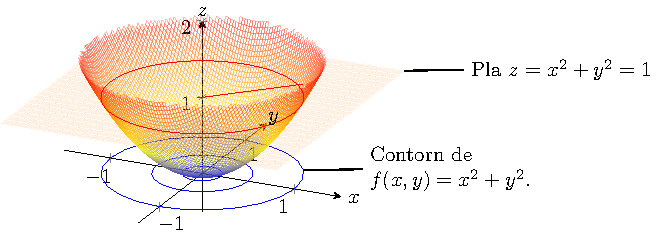
\includegraphics[width=0.9\linewidth]{paraboloid.pdf}
\end{center}

El volum del paraboloide vindria donat per l'expressió:

\[
  V=\int\int\int_{\Omega} dV 
\]

Si explorem el problema usant coordenades cartesianes, l'element de volum és $\dif V= \dif x \dif y \dif z$ i els límits d'integració quedarien com:

\[
  V=\int_{-1}^1  \int_{-\sqrt{1-x^2}}^{\sqrt{1-x^2}} \int_0^{x^2+y^2} \dif z \dif y \dif x 
\]

Podem intentar fer aquesta integral, però clarament el fet que apareguin arrels en els límits d'integració no facilita gens la feina (tot i que la integral no és pas molt complicada). Pots solucionar-la amb \texttt{Matlab} usant aquest breu codi:
\begin{lstlisting}[language=Matlab]
 syms x y z
 intZ = int(1,z,0,x^2+y^2)
 intY = int(intZ,y,-sqrt(1-x^2),sqrt(1-x^2))
 intX=int(intY)
 volum = int(intY,x,-1,1)
\end{lstlisting}

Alternativament, podem observar que la simetria de l'objecte ens permet usar coordenades cilíndriques, molt més pràctiques:

\begin{center}
  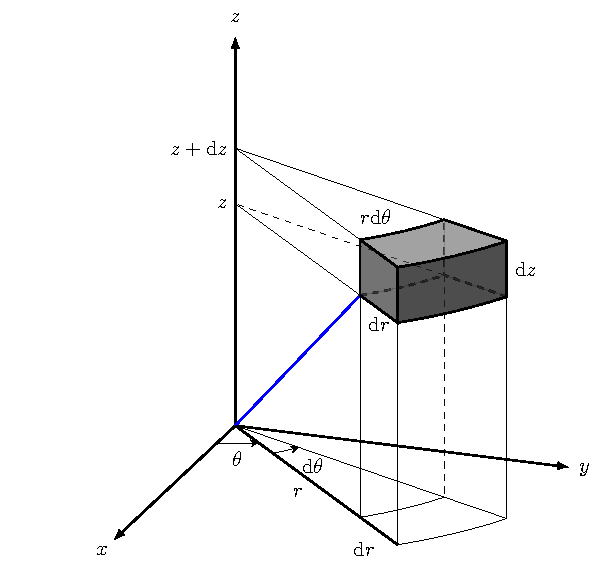
\includegraphics[width=0.5\linewidth]{CoordinatesCylindrical.pdf}
\end{center}

Ara l'element de volum vindrà donat per $\dif V = r \dif z \dif r \dif \theta$ i els límits d'integració canviaran de forma molt favorable, ja que:

\[
\begin{cases}
  -1 \leq x \leq 1\\
  -\sqrt{1-x^2} \leq y \leq \sqrt{1-x^2} \\
  0 \leq z \leq x^2 + y^2\\
\end{cases}  
\Rightarrow
\begin{cases}
  0 \leq \theta \leq 2 \pi\\
  0 \leq r \leq 1 \\
  0 \leq z \leq x^2 + y^2 = r^2\\
\end{cases}  
\]

Així:

\begin{eqnarray*}
  V&=&\int_{0}^{2\pi}  \int_{0}^{1} \int_0^{r^2} r \dif z \dif r \dif \theta = \int_{0}^{2\pi} \dif \theta  \int_{0}^{1} r \left[\int_0^{r^2} \dif z\right] \dif r \\
  &=& \theta]_{0}^{2\pi} \int_{0}^{1} r z]_0^{r^2} \dif r = 2\pi \left[\frac{r^4}{4}\right]_0^1=\boxed{\frac{\pi}{2}}
\end{eqnarray*}

%\end{Answer}
